%----------------------------------------------------------------------------------------
%	PAKET-/ UND ANDERE DOKUMENT-IMPORTS
%----------------------------------------------------------------------------------------
\documentclass[]{scrartcl}   % Formateinstellungen
\usepackage[ngerman]{babel} % deutsche Silbentrennung
\usepackage[utf8]{inputenc} % deutsche Umlaute
\usepackage{placeins}   % verbessert Anzeige eines Floats hinter dem Befehl \FloatBarrier
\usepackage{amsfonts}   % neue Schriftanpassungen (wird von amssymb (s.u.) geladen)
\usepackage{amssymb}    % erweitert Benutzung von amsfonts (s.o.)
\usepackage{amsmath}    % Vielzahl von neuen mathematischen Umgebungen und Befehlen (wird von mathtools (s.u.) geladen)
\usepackage{mathtools}  % Verbesserung von amsmath (s.o.)
\usepackage{booktabs}   % Tabellen ohne vertikale Striche
\usepackage{siunitx}    % Einheitensystem
\usepackage[margin={0.3cm,0.3cm},font=singlespacing,labelfont=bf,labelsep=endash]{caption} % Bildunterschriften
\usepackage{wrapfig}    % Bild von Text umfließen lassen
\usepackage{sidecap}    % ermöglicht Überschriften neben Bildern / Tabellen
\usepackage{setspace}   % zum Definieren des Zeilenabstandes
\usepackage{eurosym}    % ergänzt optimales Euro-Zeichen
\usepackage[perpage,marginal]{footmisc} % ermöglicht Fußnoten und das Verändern dieser
\usepackage{graphicx}   % ermöglicht besseres Einbinden von Grafiken
\usepackage{fancyhdr}   % zum Erstellen von Kopf- und Fußzeilen
\usepackage{listings}   % ermöglicht Quellcodelisting
\usepackage{color}  % Farb-Management von Vorder- und Hintergrundfarben
\usepackage{pdfpages}   % ermöglicht das Einbinden von ganzen oder nur Teilen von PDFs
\usepackage{lineno} % Zeilenzählung
\usepackage{framed} % ermöglicht das Einrahmen von Elementen
\usepackage{pifont} % fügt Symbol-Schriften hinzu
\usepackage[hidelinks]{hyperref}    % ermöglicht das Hinzufügen von Links und Verweisen innerhalb
                                    % des PDF Dokuments und weitere Einstellungen
\usepackage[left=2.5cm,right=2cm,top=2cm,bottom=2cm,includeheadfoot]{geometry}  % Größenanpassung der Seite
%----------------------------------------------------------------------------------------


%----------------------------------------------------------------------------------------
%   KONFIGURATIONEN
%----------------------------------------------------------------------------------------
\begin{document}
\setlength{\parskip}{1ex}   % Abstand zwischen Absätzen 
\parindent 0pt  % legt Einrücke der ersten Zeile fest
\renewcommand{\thefigure}{\arabic{figure}.\alph{ab}}    % Umdefinieren von Bildnummern

\definecolor{darkblue}{rgb}{0,0,.6} % Festlegen der Farben
\definecolor{darkred}{rgb}{.6,0,0}  % Festlegen der Farben
\definecolor{darkgreen}{rgb}{0,.6,0}    % Festlegen der Farben
\definecolor{red}{rgb}{.98,0,0} % Festlegen der Farben

\lstloadlanguages{Java} % lädt Programmiersprachen
\lstset{language=Java,basicstyle=\footnotesize\ttfamily,commentstyle=\itshape\color{darkgreen},keywordstyle=\bfseries\color{darkblue},stringstyle=\color{darkred},tabsize=3,showspaces=false,showtabs=false,columns=fixed,numbers=left,frame=single,numberstyle=\tiny,breaklines=true,showstringspaces=false,xleftmargin=1cm} % Erstellen eines Codeblocks
    
\pagestyle{fancy}   % Setzen des Seitenstyles "fancy" ermöglicht eigenes Erstellen einer Kopf- und Fußzeile
\fancyhf{}  % alle Kopf- und Fußzeilenfelder bereinigen
\fancyhead[L]{\leftmark}    % Kopfzeile links (mit "leftmark" erstellt man im Header das Chapter, mit "rightmark" die Section)
\fancyhead[C]{} % zentrierte Kopfzeile
\fancyhead[R]{\thepage} % Kopfzeile rechts
\fancypagestyle{plain}  % legt Seiten-Typen fest

\newcommand{\barrow}{\item[\ding{228}]} % hinzufügen des Pfeil-Aufzählsymbols unter dem Command \barrow
%----------------------------------------------------------------------------------------


%----------------------------------------------------------------------------------------
%   1. SEITE
%----------------------------------------------------------------------------------------
\titlehead{\Large

\begin{center}
\begin{framed}
\centering {Inoffizielle Lösungen und Erklärungen - \href{https://www.inf-schule.de/inf-schule}{inf-schule\textsuperscript{\textcopyright}} (\href{https://creativecommons.org/licenses/by-sa/4.0/legalcode.de}{\textit{Lizenz}})}

\centering {\Large\textbf{\href{https://inf-schule.de/programmierung/oopjava}{2.3 Objektorientierte Programmierung mit Java}}}
\end{framed}
\end{center}}

\title{\huge{\href{https://inf-schule.de/programmierung/oopjava/klassen/grundbegriffe}{1.1\\Hasen als Objekte}}\\
\vspace{0.5cm}
\begin{figure}[ht]
	\centering
	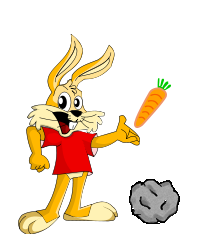
\includegraphics[height=4.5cm]{2.3.1.1/Hasen_als_Objekte.png}
\end{figure}
\vspace{2cm}}

\author{\textbf{Benötigte IDEs:}\\
\href{https://www.greenfoot.org/}{Greenfoot}, \href{https://www.bluej.org/}{BlueJ}
\vspace{2cm}}

\date{\textbf{Verfasser:}\\
\href{https://nikothegreek.jimdofree.com/}{Niko Diamadis}\\
\vspace{0.5cm}
\textbf{Erstellungs-/ Änderungsdatum}\\
\today\enlargethispage{4cm}}
%----------------------------------------------------------------------------------------

%----------------------------------------------------------------------------------------
%   2. SEITE
%----------------------------------------------------------------------------------------
\doublespacing

\maketitle\thispagestyle{empty}

\numberwithin{equation}{section}
\cleardoublepage

\setcounter{page}{1}
\tableofcontents
%----------------------------------------------------------------------------------------


%----------------------------------------------------------------------------------------
%   3. UND NACHFOLGENDE SEITEN
%----------------------------------------------------------------------------------------
\newpage
\pagenumbering{arabic}  % Ändern der Seitenangabe

\section{Objekte in Aktion}

\subsection{Objekte und Klassen}
Die gegebenen Anweisungen sollten selbsterklärend sein, hier nur noch eine passende Bildfolge dazu.

\vspace{0.3cm}

\begin{figure}[ht]
	\centering
	\includegraphics[height=4.5cm]{2.3.1.1/1.Objekte_in_Aktion/1-1.png}
	\hspace{0.5cm}
	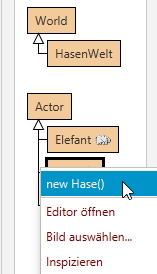
\includegraphics[height=4.5cm]{2.3.1.1/1.Objekte_in_Aktion/1-2.png}
\end{figure}

\vspace{0.5cm}

\begin{figure}[ht]
	\centering
	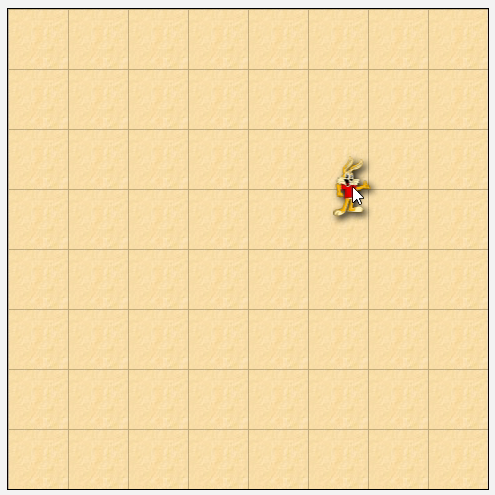
\includegraphics[height=4.5cm]{2.3.1.1/1.Objekte_in_Aktion/1-3.png}
	\hspace{0.5cm}
	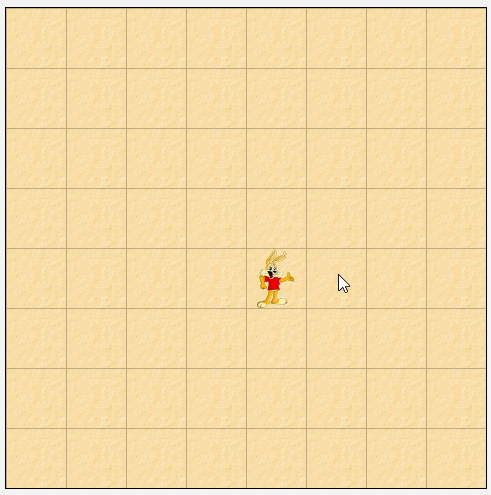
\includegraphics[height=4.5cm]{2.3.1.1/1.Objekte_in_Aktion/1-4.png}
\end{figure}

\subsection{Methoden}
Zunächst gehe ich auf die genannten Methoden eines Objektes der Klasse \texttt{Hase} ein.

\begin{itemize}
    \barrow \texttt{linksDrehen}
    \begin{itemize}
    \item der Hase dreht sich um 90$^{\circ}$ um die eigene Achse
    \end{itemize}
    \barrow \texttt{laufe}
    \begin{itemize}
    \item der Hase geht ein Feld weiter in die Richtung, in welche er gerade schaut
    \end{itemize}
    \barrow \texttt{esseKarotte}
    \begin{itemize}
    \item der Hase frisst eine Karotte, wenn beide Objekte auf einem Feld stehen
    \end{itemize}
\end{itemize}

Es folgen Bilder zur Erklärung, wie die Methoden von \texttt{Hase} und \texttt{Hasenwelt} aufgerufen werden.

\begin{figure}[ht]
	\centering
	\includegraphics[height=5.5cm]{2.3.1.1/1.Objekte_in_Aktion/2-1.png}
	\hspace{0.5cm}
	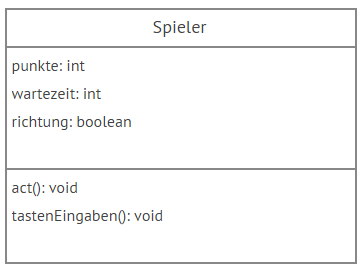
\includegraphics[height=5.5cm]{2.3.1.1/1.Objekte_in_Aktion/2-2.png}
\end{figure}

\subsection{Parameter \& Datentypen}
Nach Aufruf der Methode \texttt{setRichtung} am \texttt{Hasen}-Objekt öffnet sich ein Eingabefenster, um die gerade erlernten Parameter, welche die zu ausführende Methode, falls Parameter vorhanden, benötigt, zu übergeben.

\begin{figure}[ht]
	\centering
	\includegraphics[height=5cm]{2.3.1.1/1.Objekte_in_Aktion/3-1.png}
\end{figure}

Wie im Bild zu sehen findet man im Eingabefenster den Datentypen des Eingabewertes, der verlangt wird, in diesem Falle vom Typen \texttt{int}, also \texttt{Integer}\footnote{sprich ganzzahlige Werte von $-2^{32}$ (-2.147.483.6489) bis $2^{32} -1$ (2.147.483.647) inklusive der 0}. Zu bedenken ist jedoch, dass natürlich nicht alle Eingaben sinnvoll sind und verarbeitet werden können.\\
Selbiges gilt für die Methode \texttt{erzeugeObjekte}, nur dass dort drei Eingabewerte vom Typen \texttt{int} gefordert werden. Bei dieser Methode z.B. wird mithilfe des Eingabewertes die Anzahl der Objekte, die durch die Methode erstellt werden, festgelegt.

\begin{figure}[ht]
	\centering
	\includegraphics[height=5cm]{2.3.1.1/1.Objekte_in_Aktion/3-2.png}
	\hspace{0.5cm}
	\includegraphics[height=5cm]{2.3.1.1/1.Objekte_in_Aktion/3-3.png}
\end{figure}

\vspace{0.5cm}

\begin{figure}[ht]
	\centering
	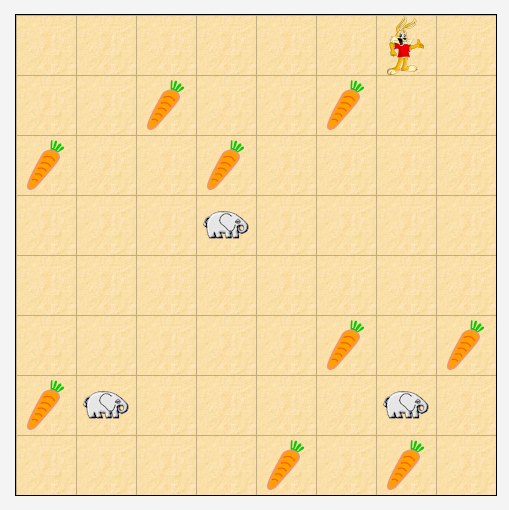
\includegraphics[height=4.5cm]{2.3.1.1/1.Objekte_in_Aktion/3-4.png}
\end{figure}

\subsection{Rückgabewerte}
Nachdem nun auch das Prinzip eines Rückgabewertes einer Methode erklärt worden ist, soll man diese an einem \texttt{Hasen}-Objekt erkunden.\\
Uns stehen bei diesem Beispiel nur zwei Methoden mit Rückgabewert zur Verfügung\\
(\texttt{int gelaufeneSchritte} und \texttt{boolean kannLaufen}; vor allen anderen steht nämlich \texttt{void}, bei diesen wird also kein Wert zurückgegeben).

\begin{figure}[ht]
	\centering
	\includegraphics[height=5cm]{2.3.1.1/1.Objekte_in_Aktion/4-1.png}
\end{figure}

Wenn man also jetzt die zurückgegebenen Werte mit den zugehörigen Signaturen abgleicht, müsste auffallen, dass beide Werte Sinn ergeben.

\newpage

\begin{figure}[ht]
	\centering
	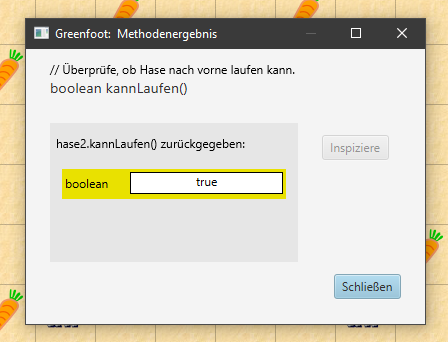
\includegraphics[height=4.5cm]{2.3.1.1/1.Objekte_in_Aktion/4-2.png}
	\hspace{0.5cm}
	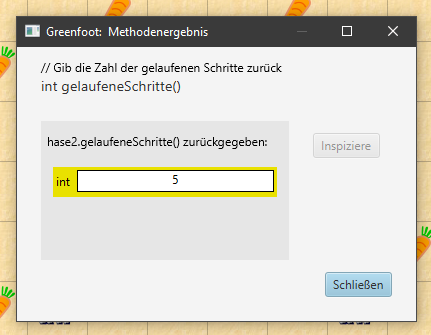
\includegraphics[height=4.5cm]{2.3.1.1/1.Objekte_in_Aktion/4-3.png}
\end{figure}

\subsection{Attribute}
Das nächste erlernte Konzept ist das der Attribute.\\
Das geforderte Inspizieren eines Objektes ist ganz einfach durch einen Rechtsklick auf irgendeines der Objekte und das Auswählen von \glqq Inspizieren\grqq{} möglich.

\begin{figure}[ht]
	\centering
	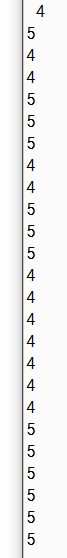
\includegraphics[height=10cm]{2.3.1.1/1.Objekte_in_Aktion/5-1.png}
\end{figure}

Die als Beispiel gesuchten Attribute für die Position des Objektes sind \texttt{int x} und \texttt{int y}.

\newpage

\subsection{Quelltext}
Zu dieser Aufgabe sind meines Erachtens nach keine Anleitungen und/oder Erläuterungen nötig.\\
Wenn doch Fragen aufkommen, schreib' einfach an \textbf{\href{mailto:nikodiamond3@gmail.com}{nikodiamond3@gmail.com}}.

\subsection{Vererbung}

Die markierten Methoden sind die von \texttt{Actor} vererbten Methoden, alle, welche unter \glqq geerbt von Actor\grqq{} stehen, sind in der Klasse \texttt{Hase} selbst definiert.\\

\begin{figure}[ht]
	\centering
	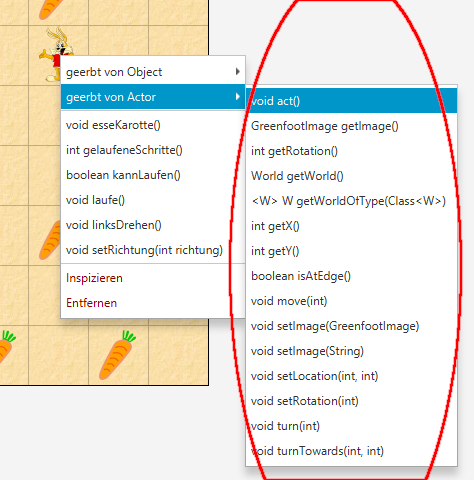
\includegraphics[height=9.5cm]{2.3.1.1/1.Objekte_in_Aktion/7-1.png}
\end{figure}

Analog funktioniert es auch mit der Klasse \texttt{Elefant}.

\newpage
\subsection{Klassendiagramm für Hase}

Ganz oben im Klassendiagramm steht der Klassenname.\\
Darunter lassen sich die Attributnamen und dahinter deren Datentyp finden.

Ganz unten findet man die Methoden und angehängt deren Rückgabetyp. Die Parameter werden direkt hinter dem Methodennamen in Klammern angegeben (auch hier zuerst Variablennamen und dann der Datentyp).\\

Anschließend folgen noch die geforderten Ergänzungen im Klassendiagramm.\\

\begin{figure}[ht]
	\centering
	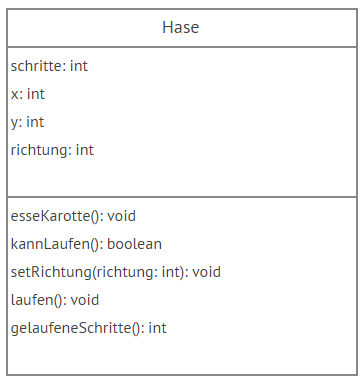
\includegraphics[height=9.5cm]{2.3.1.1/1.Objekte_in_Aktion/8-1.png}
\end{figure}

\newpage

\section{Fachkonzept - Objekt}
Zu dieser Seite sind meines Erachtens nach keine Anleitungen und/oder Erläuterungen nötig.\\
Wenn doch Fragen aufkommen, schreib' einfach an \textbf{\href{mailto:nikodiamond3@gmail.com}{nikodiamond3@gmail.com}}.

\newpage

\section{Fachkonzept - Klasse}
Zu dieser Seite sind meines Erachtens nach keine Anleitungen und/oder Erläuterungen nötig.\\
Wenn doch Fragen aufkommen, schreib' einfach an \textbf{\href{mailto:nikodiamond3@gmail.com}{nikodiamond3@gmail.com}}.

\newpage

\section{Übungen}

\subsection{Geburtstagsrechner}

Hier folgt die Struktur der Beispielsklasse \texttt{Person}.

\begin{itemize}
    \barrow Attribute
    \begin{itemize}
    \item \texttt{tag} vom Datentypen \texttt{int}
    \item \texttt{monat} vom Datentypen \texttt{int}
    \item \texttt{jahr} vom Datentypen \texttt{int}
    \item \texttt{name} vom Datentypen \texttt{String}
    \end{itemize}
    \barrow \texttt{Methoden}
    \begin{itemize}
    \item \texttt{getAlter} mit \texttt{int} als Rückgabewert und ohne Parameter
    \item \texttt{getTageBisGeburtstag} mit \texttt{int} als Rückgabewert und ohne Parameter
    \item \texttt{setGeburtstag} ohne Rückgabewert und mit den Parametern \texttt{int t}, \texttt{int m}, \texttt{int y}
    \item \texttt{istVolljaehrig} mit \texttt{boolean} als Rückgabewert und ohne Parameter
    \item \texttt{setName} ohne Rückgabewert und mit dem Parameter \texttt{String name}
    \item \texttt{druckeInfo} ohne Rückgabewert und ohne Parameter
    \end{itemize}
\end{itemize}

\vspace{0.5cm}

\begin{figure}[ht]
	\centering
	\includegraphics[height=4.5cm]{2.3.1.1/4.Uebungen/1-1.png}
\end{figure}

\newpage

Im Screencast wurden folgende Schritte ausgeführt:

\begin{itemize}
    \barrow Erstellen zwei neuer Objekte der Klasse \texttt{Person} mit den Namen \texttt{a} und \texttt{b}
    \barrow Inspizieren des Objektes \texttt{a}
    \barrow Aufrufen der \texttt{setName}-Methode an \texttt{a} mit dem Parameter \texttt{name = \dq Anna"}
    \barrow Aufrufen der \texttt{setGeburtstag}-Methode an \texttt{a} mit den Parametern \texttt{geburtsTag = 10},\\ \texttt{geburtsMonat = 4} und \texttt{geburtsJahr = 2000}
    \barrow Aufrufen der \texttt{getAlter}-Methode an \texttt{a}
    \barrow Aufrufen der \texttt{istVolljaehrig}-Methode an \texttt{a}
    \barrow Aufrufen der \texttt{getTageBisGeburtstag}-Methode an \texttt{a}
    \barrow Aufrufen der \texttt{druckeInfo}-Methode an \texttt{a}
\end{itemize}

\subsection{Zusammenfassung der Begriffe}

\begin{table}[ht]
\centering
\begin{tabular}{c|p{10cm}}
	\\Begriff & Definition\\
	\hline
	
	\\Klasse & Eine Klasse ist ein Bauplan für Objekte. Dieser Bauplan legt genau fest, welche Attribute die zu konstruierenden Objekte haben sollen und welche Methoden sie ausführen können sollen.\\
	
	\\Objekt & Ein Objekt ist eine Einheit, die Daten mit Hilfe von Attributen verwalten und Operationen zur Verarbeitung der verwalteten Daten mit Hilfe von Methoden ausführen kann.\\

	\\Attribut & Attribute sind - an Objekte gebundene - Variablen zur Verwaltung von Daten. Diese entsprechen in der Regel den Eigenschaften der betreffenden Objekte.\\

	\\Methode & Methoden sind - an Objekte gebundene - Fähigkeiten zur Verarbeitung von Daten. Diese Methoden werden ausgeführt, wenn das betreffende Objekt veranlasst wird, eine bestimmte Operation auszuführen.\\
\end{tabular}
\end{table}

\newpage

\begin{table}[ht]
\centering
\begin{tabular}{c|p{10cm}}
    \\Parameter & Parameter sind Variablen, die dazu dienen, einer Methode beim Aufruf bestimmte Informationen zu übergeben.\footnotemark\\

    \\Rückgabewert & Rückgabewerte sind diejenigen Werte, welche von Methoden als Antwort geliefert werden.\\

	\\Datentyp & Ein Datentyp gibt an, welche Art von Information ein Attribut hält.\\
	
	\\Signatur & Eine Signatur einer Methode gibt den Rückgabewert, den Namen und die Parameter einer Methode an.\\

	\\Vererbung & Die Vererbung ist eine Vorgehensweise, um von einer Klasse ausgehend eine Unterklasse definieren zu können, welche alle Attribute und Methoden der Überklasse übernimmt und auch abrufen kann.\\

	\\Klassendiagramm & Ein Klassendiagramm ist ein Hilfsmittel, um Klassen inklusive ihrer Attribute und Methoden und deren Beziehungen einfach und übersichtlich darzustellen. Meist sind diese Diagramme in der \texttt{Unified Modelling Language (UML)} geschrieben.\\

	\\Objektdiagramm & Ein Objektdiagramm ist ähnlich aufgebaut wie ein Klassendiagramm, nur dass der Name des beschriebenen Objektes dargestellt wird, anstatt der Datentypen Werte eingesetzt sind und meist die Methoden weggelassen werden, da diese bereits im Klassendiagramm wiederzufinden sind.\\
\end{tabular}
\end{table}

\footnotetext{Parameter, Informatik, https://www.u-helmich.de/inf/BlueJ/lexikon/M-R/Parameter.html, (Abgerufen: 24.02.20, 00:22)}

\newpage

\begin{figure}[ht]
    \centering
	\includegraphics[height=10cm]{2.3.1.1/4.Uebungen/2-1.png}
\end{figure}

Den Screencast lasse ich aus, das kannst du ja selber erledigen, wenn du es noch machen möchtest.

\newpage

\subsection{Klassen- und Objektdiagramme}

\begin{figure}[ht]
    \centering
	\includegraphics[height=11cm]{2.3.1.1/4.Uebungen/3-1.png}
\end{figure}

\vspace{0.5cm}

\begin{figure}[ht]
	\centering
	\includegraphics[height=5.5cm]{2.3.1.1/4.Uebungen/3-2.png}
	\hspace{0.5cm}
	\includegraphics[height=5.5cm]{2.3.1.1/4.Uebungen/3-3.png}
\end{figure}

\newpage

\subsection{Kreuzworträtsel}

\begin{figure}[ht]
    \centering
	\includegraphics[height=13.5cm]{2.3.1.1/4.Uebungen/4-1.png}
\end{figure}

\end{document}
